Standard LoRa (nazwa pochodzi od słów "Long Range") należy do grupy systemów z~rozproszonym widmem (ang.
\textsl{Spread~Spectrum}) bazującą na technice \textsl{Chirp Spread Spectrum} (CSS). Wykorzystuje ona szerokopasmowe
impulsy typu \enquote{chirp} modulowane liniową częstotliwością w~celu kodowania przesyłanych informacji. Sygnał
jest sinusoidą, której częstotliwość wzrasta (\enquote{Up-Chirp}) lub maleje (\enquote{Down-Chirp}) w~czasie
\cite{semtech-lora-lorawan,ieee-802-15-4-2006}.

Wykorzystanie LoRa pozwala na budowanie sieci, które mogą transmitować na duże odległości, zużywając przy tym małe
ilości energii. Zaprojektowana z~myślą o~urządzeniach wykorzystujących zasilanie bateryjne w~celu podłączenia ich
bezprzewodowo do lokalnych, regionalnych lub globalnych sieci. Standard wykorzystuje transmisje na bezlicencyjnych
częstotliwościach radiowych poniżej 1~GHz -- przykładowo w~Europie jest to 868 MHz (EU868), natomiast w~Ameryce
Północnej 915 MHz (US915). Sama implementacja technologii obejmuje tylko warstwę fizyczną (najniższą, najbliżej
bezpośredniego połączenia pomiędzy urządzeniami, LoRaPHY), jednakże dostępne są także protokoły obejmujące warstwy
wyższe -- przykładowo LoRaWAN (ang. \textsl{Long Range Wide Area Network}).

\section{\label{sect:loraphy}Warstwa fizyczna -- LoRaPHY} Podstawą standardu LoRa jest jego warstwa fizyczna (PHY),
która opiera się na modulacji widma rozproszonego pochodnej od \textsl{Chirp Spread Spectrum} (CSS). W~modulacji LoRa
rozproszenie widma uzyskiwane jest dzięki generowaniu sygnałów typu chirp, które posiadają ciągłą zmianę w~ich
częstotliwości. Przy wykorzystaniu takiej metody przesunięcia w~czasie oraz częstotliwości są identyczne dla nadajnika,
jak i~odbiornika, dzięki czemu złożoność konstrukcji odbiornika może być znacznie zredukowana
\cite{lora-modulation-basics}.

W~przypadku wykorzystania warstwy fizycznej LoRaPHY możliwe jest zbudowanie sieci bazującej na połączeniu radiowym
urządzenie-urządzenie (D2D, ang. \textsl{device to device}), gdzie dwa urządzenia komunikują się bezpośrednio między
sobą. W~takim układzie przeważnie jedno z~nich jest inicjującym wymianę danych poprzez wysłanie zapytania, natomiast
drugie po odebraniu go wysyła odpowiedź. Moduły takie są często nazywane odpowiednio modułami MASTER oraz SLAVE.

Jedna ramka transmisji LoRa składa się z~ciągu zmodulowanych symboli $s(nT_s)$, zgodnie z~zależnością
\cite{lora-modulation-fscm,lora-emulator}:
\begin{equation}
    x(t) = \sum_{n=1}^{N_M} s_n(t-nTs)\text{,}
\end{equation}
gdzie $N_m$ jest całkowitą ilością symboli w~przesyłanej ramce.

\subsection{\label{sect:lora-modulation}Modulacja LoRa -- LoRa Spread Spectrum} Modulacja LoRa bazuje na cyklicznych
(powtarzających się) sygnałach typu chirp (tzw. \enquote{świergotach}), a~przesunięcia częstotliwości w~stosunku do
częstotliwości nośnej, czyli \enquote{pozycja startowa} pozwala na zakodowanie wartości symbolu. Parametrem pozwalającym
na kontrolę częstotliwości chirpów jest \textsl{speading factor} ($\mathrm{SF}$). W~przypadku regionu europejskiego
wartość ta może zostać wybrana z~przedziału \{7,8,9,10,11,12\}. Im większa jego wartość, tym dłużej trwa przesłanie
jednego sygnału, co w~efekcie pozwala na przesłanie większej ilości bitów w~jednym symbolu. Jeden chirp
(\enquote{świergot}) w~standardzie LoRa zaprojektowany został do odzwierciedlenia $M=2^{\mathrm{SF}}$ wartości symboli,
gdzie ich czas trwania (długość) dana jest w~postaci $T_s=M/\mathrm{BW}$, a~wartość $\mathrm{BW}$ przedstawia
wykorzystaną szerokość pasma \cite{lora-modulation-fscm}. LoRa wykorzystuje zadane wartości szerokości pasma,
z~przedziału $\mathrm{BW}$=\{125,250,500\} kHz, przy czym ich dostępność zależna jest od tego, gdzie sieć operuje i~jest
regulowana \cite{lora-regional-parameters}, tak samo, jak inne parametry sieci, przez LoRa Alliance. Zmodulowany przez
LoRa przebieg można przedstawić analitycznie w~postaci \cite{lora-emulator}:
\begin{equation}\label{eqn:lora-waveform}
    s(t) = \exp{\left({j}2\pi\int_{0}^{t}\left[(\beta x+\gamma_n)_{\bmod{_{\mathrm{BW}}}}-\frac{\mathrm{BW}}{2}\right]\,dx\right)}\text{,}
\end{equation}
gdzie $\gamma_n$ to przesunięcie częstotliwości, które można wyznaczyć, korzystając z~zależności:
\begin{equation}
    \gamma_n = m_n\Delta_f = \frac{m_n}{T_s}\text{,}
\end{equation}
gdzie $m_n$ jest wartością symbolu z~przedziału $m_n\in\{0,1,\ldots,M-1\}$, $n$ jest indeksem symbolu, a $\Delta_f$
przedstawia krok między zmianami częstotliwości.

W~przypadku LoRa krok w~zmianie częstotliwości wybrany został jako częstotliwość pojedynczego symbolu $B/M$. Kolejnym
ważnym dla modulacji LoRa parametrem jest tzw. \enquote{częstotliwość świergotania} (ang. \textsl{Chirp Rate}).
Odpowiednio dobrany, pozwala na separację symboli oraz uniknięcie zakłóceń międzysymbolowych (ISI, ang.
\textsl{Inter-Symbol Interference}). Wyznaczany jest na podstawie czasu trwania jednego symbolu $T_s$ w~danym paśmie
transmisyjnym $\mathrm{BW}$, tak aby każdy symbol zaczynał się oraz kończył na takiej samej częstotliwości:
\begin{equation}
    \beta = \frac{f_{\mathrm{high}}-f_{\mathrm{low}}}{T_s}=\frac{\mathrm{BW}}{T_s}\text{,}
\end{equation}
gdzie $f_{\mathrm{high}}\ \text{oraz}\ f_{\mathrm{low}}$ to odpowiednio górna i~dolna granica częstotliwości
pojedynczego świergotu. W~przypadku, gdy wartość $\beta > 0$, sygnał będzie typu upchirp (o częstotliwości rosnącej),
natomiast typu downchirp (o częstotliwości malejącej) dla $\beta < 0$. Reprezentacja dwóch symboli LoRa
\cite{lora-emulator} przedstawiona zotała na rys. \ref{img:upchirp-lora-modulated-symbol}. Dzięki zastosowaniu takiej
modulacji, energia sygnału rozproszona jest w~większym paśmie transmisyjnym, co pozwala na znaczne zredukowanie
wąskopasmowych zakłóceń (ang. \textsl{narrow-band interferences}). W~przypadku, gdy do transmisji wybrana zostanie
wyższa wartość SF, zwiększa się czułość odbiornika z~uwagi na zwiększoną energię symbolu, jednakże skutkuje to
zmniejszeniem przepustowości sieci oraz zwiększonym zużyciem energii przez moduły \cite{css-modulation-technique}.

\begin{figure}[!htbp]
    \centering
    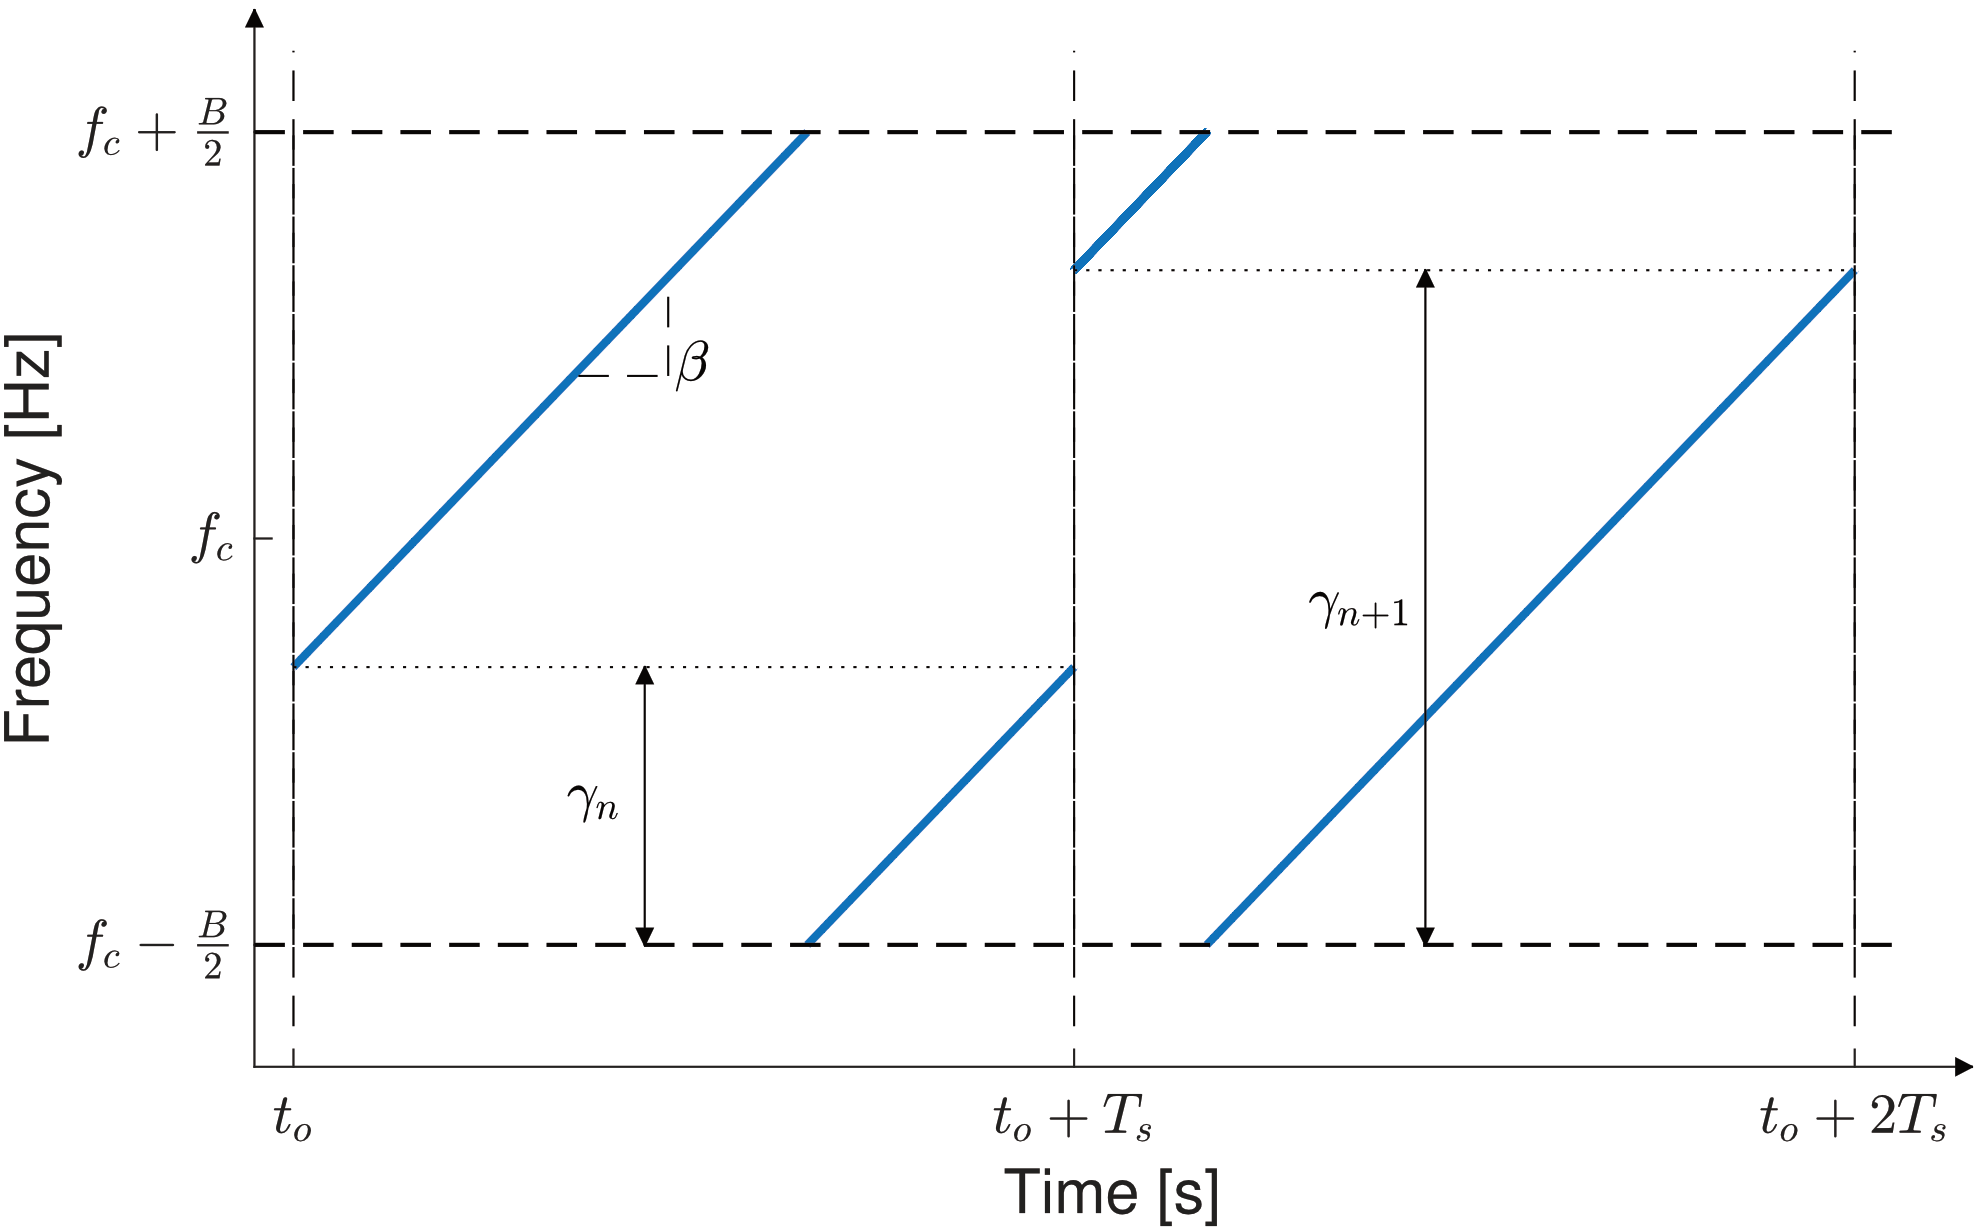
\includegraphics[width=0.9\textwidth]{theory/upchirp-lora-modulated-symbol}
    \caption{\label{img:upchirp-lora-modulated-symbol}Przebieg dwóch symboli typu upchirp w~modulacji LoRa, ilustracja
        wykorzystana zgodnie z licencją publikacji \cite{lora-emulator}}
\end{figure}

\FloatBarrier
\section{\label{sect:lorawan}Wyższe warstwy -- protokół LoRaWAN}
\begin{figure}[!htbp]
    \centering
    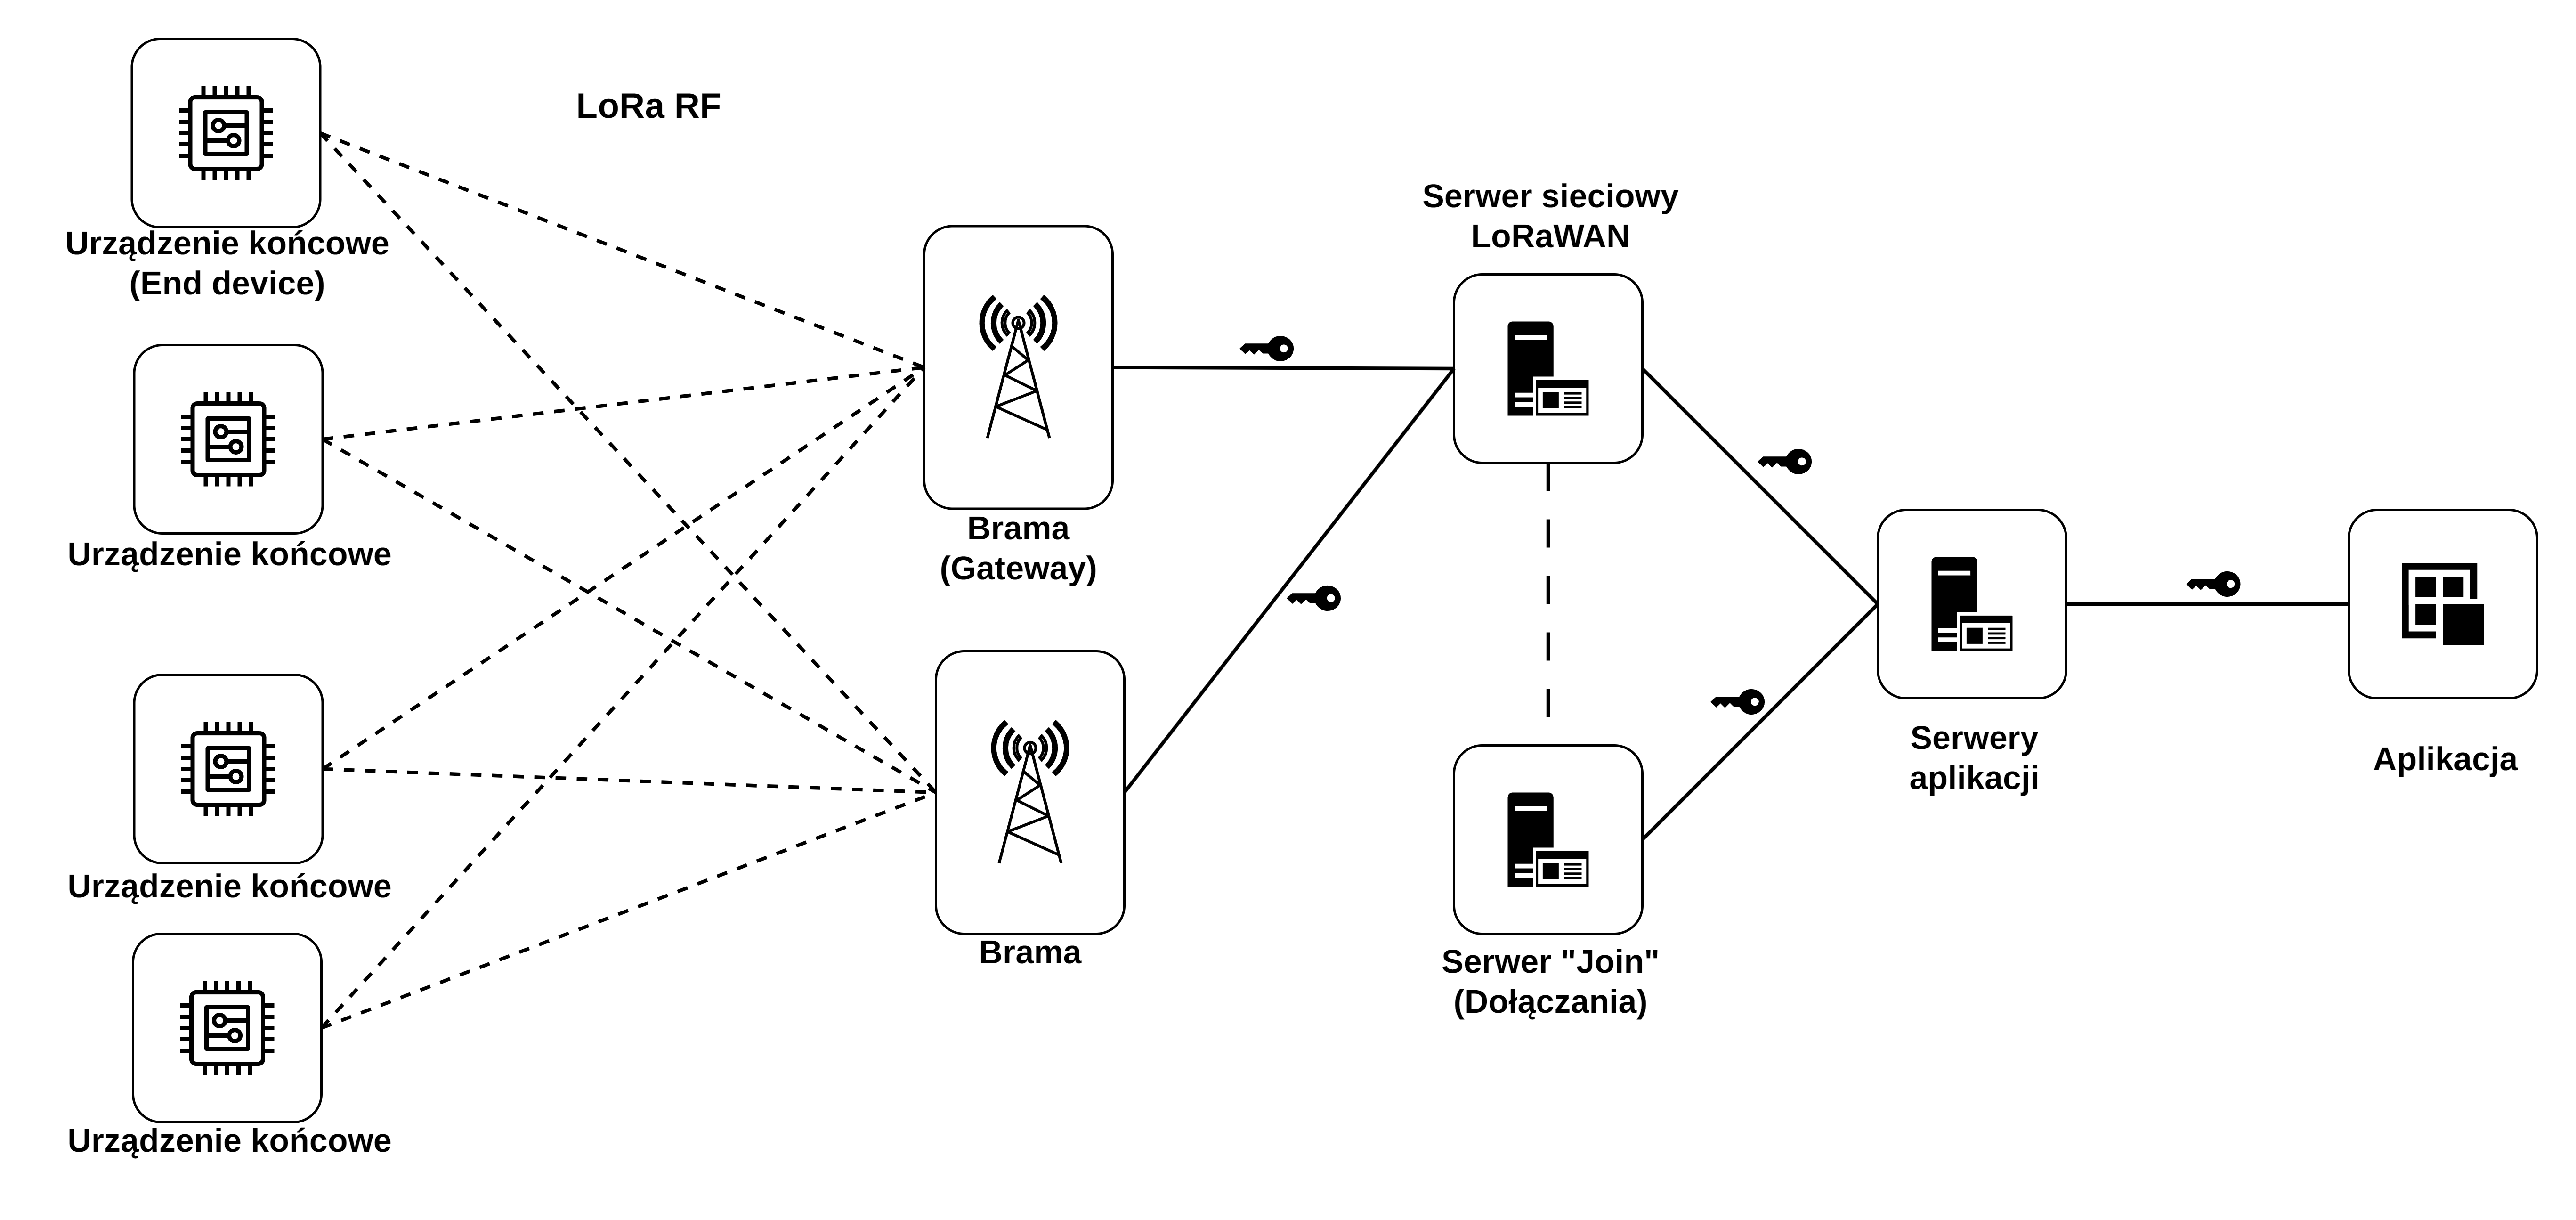
\includegraphics[width=\textwidth]{schematics/lorawan-architecture}
    \caption{\label{img:lorawan-architecture}Schemat architektury sieci LoRaWAN}
\end{figure}